\documentclass[sigconf]{acmart-txmm}

\usepackage{booktabs} % For formal tables
\usepackage{url}
\usepackage{color}
\usepackage{enumitem}
\usepackage{lscape}
\usepackage{graphicx}
\usepackage{float}

\hyphenation{Media-Eval}

% Copyright
%\setcopyright{none}
%\setcopyright{acmcopyright}
%\setcopyright{acmlicensed}
\setcopyright{rightsretained}
%\setcopyright{usgov}
%\setcopyright{usgovmixed}
%\setcopyright{cagov}
%\setcopyright{cagovmixed}

% DOI
\acmDOI{}

% ISBN
\acmISBN{}

%Conference
\acmConference[TxMM'18-'19]{Text and Multimedia Mining}{Radboud University}{Nijmegen, Netherlands} 
\acmYear{}
\copyrightyear{}

\acmPrice{}

\begin{document}
\title{Trading Bitcoin based on Tweets}

\author{J.M. van Hulst}
%%\authornote{The secretary disavows any knowledge of this author's actions.}
\affiliation{Radboud University, Nijmegen, Gelderland}
\email{mick.vanhulst@gmail.com}

\renewcommand{\shortauthors}{J.M. van Hulst}
\renewcommand{\shorttitle}{Twitter based Bitcoin trading}

\begin{abstract}
This paper introduces a method that can be used for trading Bitcoin. It is based on specific word usage within Twitter messages (also known as 'Tweets') by Twitter users. The goal of this research is to show if predictions regarding the Bitcoin price can be made by utilizing textual relationships of Tweets for specific users and if user-specific information carries importance when making such predictions. We instantiate matrices that are specific to a user's Tweets over a set amount of time. These matrices are used to train a Convolutional Neural Net (CNN), which predicts whether or not a profitable trade can be made. Keywords are found by using TF-IDF, which is a general technique that iss used for finding words of importance in a set of documents (i.e. Tweets in our case).  The user-specific results are aggregated by day, resulting in a single prediction per day by utilizing a Logistic Regression (LR) and arithmetic mean based method. Success is measured by calculating the Precision and Recall scores. These scores are related to the, assumed to be goal of the trader, which is to increase its overall capital. The results show that it is preliminary to say whether or not the method is of significance to a trader, but the work aims to serve as a baseline for future research.
\end{abstract}

\maketitle

\section{Introduction}
\label{sec:intro}
In 2008 the peer-to-peer electronic cash system called Bitcoin was introduced by Satoshi Nakamoto \cite{Nakamoto_bitcoin:a}. In the following years, Bitcoin increased in value and popularity. With the increasing popularity of social media, one would assume that the popularity of Bitcoin would be expressed on social media. Kaminski \cite{1406.7577} suggests that the Twitter platform may be interpreted as a virtual trading floor that emotionally reflects Bitcoin's market movement, but his results show that Twitter sentiment is not predictive for Bitcoin market movement. Rather than focusing on the sentiment of Twitter, this work focuses on specific keyword usage of Twitter users overtime, such that models can be trained to predict whether or not a profitable trade can be made.

The model that this work focuses on is called a CNN. CNNs have previously been used for problems where the data consisted of spatial relationships such as AlexNet, a CNN that predicted class labels of (ImageNet) images \cite{NIPS2012_4824}. The structure of a CNN, however, can also be changed to a one-dimensional sequence. This allows the CNN to be used more generally on other types of data that have a spatial relationship. For example, there is an ordered relationship in the time steps of a time series \cite{machine_learning_mastery_2018}. The problem that is tackled in this work also consists of a time series, which is why one-dimensional CNNs are utilized. This allows for the possibility of finding patterns in the usage of words for specific users at certain time intervals.

The objective of this work is to find if it is possible to develop a model for predicting profitable trades based on specific Twitter users their messages. Furthermore, focusing on a specific set of Twitter users makes room for the usage of user specific meta-data, such as the amount of followers, which might hold meaning when predicting profitable trades based on user-specific Tweets. This work aimed to answer the following questions:
\begin{enumerate}
    \item Can a set of Tweets from specific Twitter users be used to predict profitable trades for Bitcoin?
    \item Does the predictive value of the aforementioned model increase when utilizing meta-data of this specific set of users?
\end{enumerate}

\section{Related work}
\label{sec:related}
As mentioned in the introduction, Kaminski \cite{1406.7577} concludes that the Twitter platform may be interpreted as a virtual trading floor that emotionally reflects Bitcoin's market movement. However, Kaminski performed a dynamic Granger causality analysis and reports that it does not confirm a causal effect of emotional Tweets on Bitcoin market values, meaning that Twitter sentiment does not precede changes in Bitcoin market values. Hernandez et al. \cite{inproceedings}, in their work, explain that Twitter users that are interested in Bitcoin are less likely to use emotional related words in their Tweets. Sul et al. \cite{sul2017trading}, when predicting stock returns, find that sentiment of Tweets coming from users with many followers had no significant impact on the return of a stock and they observed the opposite when users had fewer followers. Although their work focused on the stock market, this could be an indication that user meta-data (e.g. amount of followers), is of importance when measuring price changes. The combination of this previous work raised the idea of focusing this work on predicting profitable trades for Bitcoin by focusing on a fixed set of Twitter users, such that meta-data can be used, and instead of relying on Twitter sentiment, relying on the Twitter users their word-usage over a fixed time interval such that predictions can be made based on word usage patterns.

Previous work regarding the development of models for trading include Hoseinzade et al. \cite{1810.08923} their work, which focused on using CNNs to predict the next day's movement of certain indices of S&P 500, NASDAQ, DJI, NYSE, and RUSSELL markets by using various features such as the RSI (Relative Strength Index). 
For Bitcoin specific trading, Hotz-Behofsits et al. \cite{1801.06373} developed non-Gaussian state space models and focused on the daily change in the log price of Bitcoin, Ethereum and Litecoin. They developed a simple trading strategy for the optimization of portfolio allocation. For Bitcoin specific trading there is one interesting mention that, according to their results, achieved great success. This paper was released by Devavrat et al. \cite{1410.1231}, and used data coming from the order book of the exchange 'Okcoin.com' to perform Bayesian regression such that the model gave indications as to whether or not they should buy, sell or hold Bitcoin. After 60 days, they mention to have doubled their investment. 

\section{Approach}
\label{sec:approach}
\subsection{Data}
\subsubsection{Data Gathering}
\label{sec:data_gath}
The method for gathering data that is used in this work is based on prior work done by Sul et al. \cite{sul2017trading}. Their work mentions that Twitter users use a dollar sign and a shortcut of a certain stock as an indication that they are Tweeting about a particular stock. In the case of this work, this means that Tweets are collected that contain '\$btc' (not capital letter sensitive). Collecting Twitter data consisted of using Tweepy (a Python package) \cite{tweepy_2018}, and after collecting data between the period of 26th of September (2018) to the 2nd of January (2019), the Tweets were processed and a list of unique usernames was generated. Iterating over each user and gathering all their Tweets that contained the aforementioned keyword resulted in the final dataset\footnote{This approach was used due to Twitter limiting access to historical data when using specific keywords (i.e. scraping can be done up to 14 days back in time)}. The resulting Tweets were preprocessed by removing Retweets, Tweets with more than one ticker symbol sign\footnote{According to Sul et al. \cite{sul2017trading} multiple ticker symbols makes it hard to differentiate between which subject a message is about. Meaning a combination of e.g. \$ETH for Ethereum and \$BTC for Bitcoin in one message makes it unclear as to which one of the tickers the Tweet is about.}, URLs, mentions, excessive characters (e.g. 'goood' is transformed to 'good'), unicode characters, stopwords, digits that indicated a price and punctuations. Lastly, all characters were converted to lower-case characters and all Tweets prior to June 1st 2017 were removed. Figure \ref{fig:dist_Tweets} shows the final distribution of the entire dataset before splitting the dataset into a training and test set. Before splitting, the data was ordered such that a clear temporal cut could be made. The test data consisted of the last two months of data (1st of November 2018 to the 2nd of January 2019). This allowed for making predictions in the 'future' as the data in the data coming from dates in the test set lied ahead in time with respect to the training data. The total amount of Tweets for the training set equaled 190.038 and the total amount of Tweets for the test set equaled 62.644, where all users that were not both in training and test data were removed.

\begin{figure}[H]
  \centering
  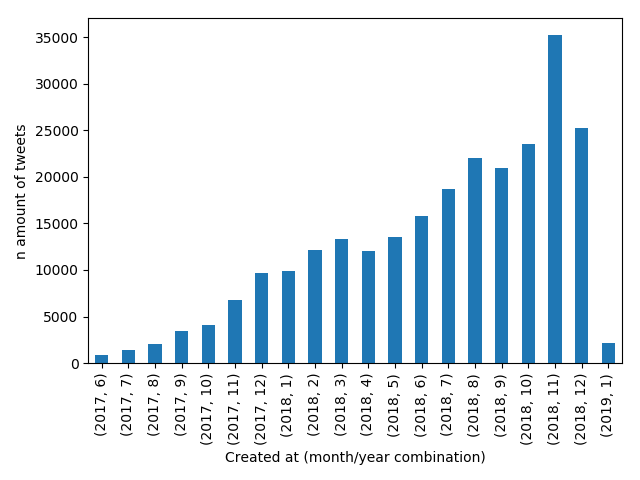
\includegraphics[width=0.75\linewidth]{report/img/distribution_tweets.png}
  \caption{Distribution of final set of Tweets per month and year combination.}
  \label{fig:dist_Tweets}
\end{figure}

Besides Tweets, users their meta-data was also retrieved using the aforementioned package Tweepy. As a user's meta-data changes overtime (e.g. people gain more followers), only the most recent meta-data for a particular user was used for the experiments. The set of meta-data consisted of: If the user's account was verified or not, the amount of followers the user had, amount of accounts the user followed, the amount of public lists the user was in, total amount of Tweets the user liked, number of Tweets created by the user, the time the account user has existed for expressed in months and the user's twitter ID.

To determine whether or not a trade would have been profitable for a particular day, the Bitcoin closing price of a day prior to that day was subtracted from the Bitcoin closing price of that particular day. A fee was then applied to the resulting value that has to be paid when making a trade. If the resulting calculated value was positive, then the trade would have been profitable, else it would not have been profitable. Bitcoin price information was retrieved from CryptoDataDownload \cite{cryptodatadownload}, which is a platform that aims to provide free historical data for several cryptocurrencies. As Bitcoin prices can differ per platform, this work focused on Coinbase's price fluctuations and thus their fees were applied in the aforementioned calculation \cite{coinbase_pro}.

\subsubsection{Matrices}
\label{sec:matrices}
CNNs require a matrix as input, where the goal is that the matrix captures some form of a pattern that can be used as an indicator for the class that it represents. The matrices existed of the amount of features as rows and the amount of timesteps as columns. These features were derived from Tweets, where Tweets contained words and/or specific characteristics that were informative for prediction profitable trades. This way, a time series was created that captured the change in features (i.e. word usage) for a specific amount of timesteps.

First, TF-IDF was used to generate the importance of specific words with respect to the entire set of training tweets. Second, the top 500 words with the highest TF-IDF scores were used as individual rows for the matrices. Third, the amount of columns for a matrix was fixed to 7, meaning that a matrix's shape consisted of 500 rows by 7 columns. Fourth, Tweets were represented in the aforementioned matrices by processing Tweets for specific users of specific dates and seeing whether or not the top 500 TF-IDF generated words occurred in a Tweet for a specific date. To create a single matrix, this last step was repeated 7 times for each date for a specific user. The final matrix captured the change in specific word usage for a user over a period of 7 days. Using the aforementioned method, four types of matrices were created. The first matrix was a binary matrix consisting of zeroes and ones, where ones represented a TF-IDF word occurring in a Tweet for a specific user and date combination, and where a one meant that there was a full match between a word in the Tweet and a word in the TF-IDF generated list (i.e. meaning that the word 'fear' only matches 'fear' and not 'fearful). The second type of matrix was similar to the previous matrix, but instead of being binary, it counted the occurrences of a word in a tweet, meaning that matrices did not solely consist of zeroes and ones. The third and fourth matrix were similar to the aforementioned matrices, but used partial matching, meaning that a word such as 'fear' also matched 'fearful' as 'fear' is a subword of 'fearful'. Figure \ref{fig:ex_matrix} shows an example of a binary matrix for partial matching, where the x-axis represents the columns (i.e. 7 days) and the y-axis represents the number of features (i.e. TF-IDF words), and where the occurrences of a word are represented by a black stripe. Throughout this work partial matching will be referred to as 'Partial TF-IDF' and full matching will be referred to as 'TF-IDF'.

\begin{figure}[H]
  \centering
  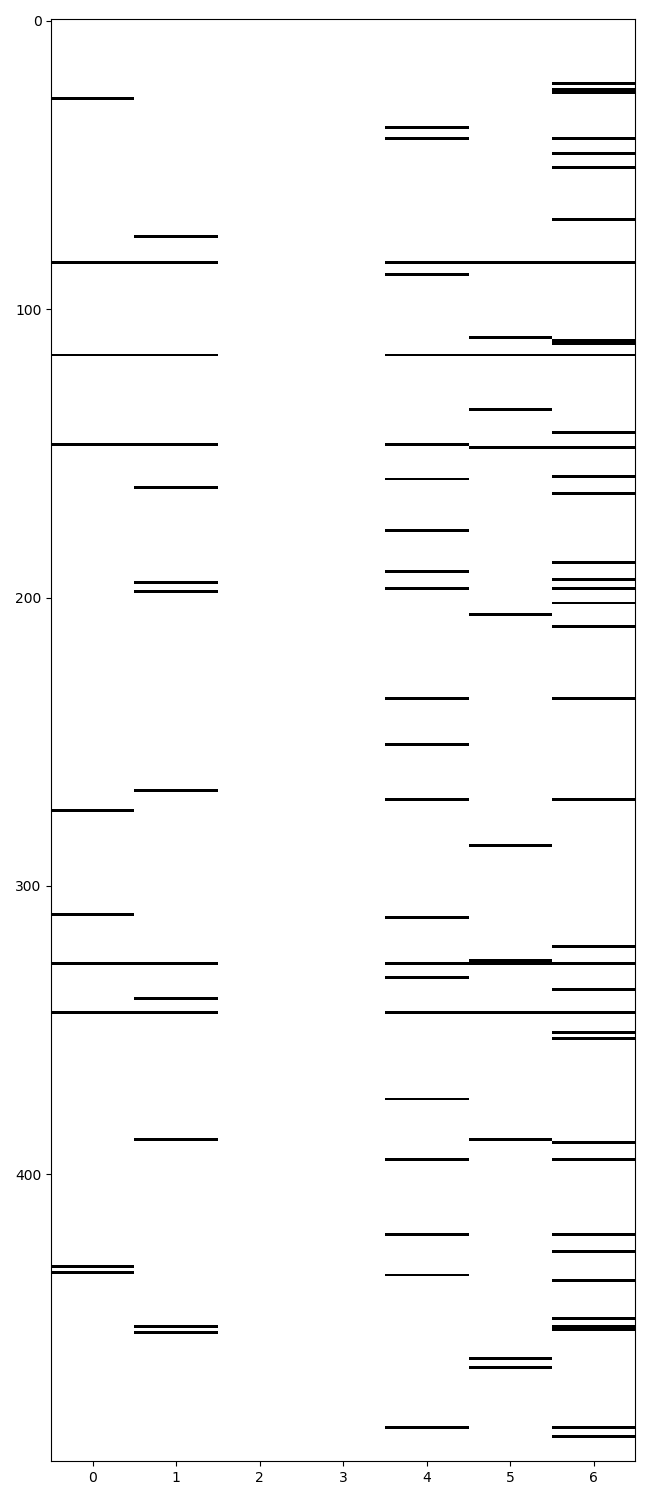
\includegraphics[width=0.5\linewidth]{report/img/binary_train_0_28500.png}
  \caption{Example binary matrix for partial matching.}
  \label{fig:ex_matrix}
\end{figure}

User meta-data and classes were not processed in matrices as this did not include a spatial relationship. User meta-data was concatenated in the network, which will be discussed in the next section. The labels the models were trained on were created by storing whether or not a trade would have been profitable the day after the last day of the matrix\footnote{Meaning that if a matrix consisted of columns between t-7 and t, where t was an arbitrary date, the class consisted of if the trade would have been profitable at t+1.}. As a last step, all matrices and users their meta-data were normalized.

Table \ref{table:n_matrices} shows the total amount of matrices that were gathered per type of matrix representation. One can observe that the amount of matrices per representation differs, which is due to matrices only being non-zero if the TF-IDF words occurred in a Tweet.

% Please add the following required packages to your document preamble:
% \usepackage{booktabs}
% \usepackage{graphicx}
\begin{table}[H]
\centering
\caption{Size of training and test set for each model.}
\label{table:n_matrices}
\begin{tabular}{@{}lll@{}}
 & \textbf{Train} & \textbf{Test} \\
\toprule
\textbf{Partial TF-IDF} & 126.949 & 35.750 \\
\textbf{TF-IDF} & 24.278 & 7.003 \\ 
\bottomrule
\end{tabular}%
\end{table}

\subsection{Models}
This section introduces the methods that were used for predicting profitable trades for Bitcoin. Making a prediction for a particular date consisted of two steps. The first step consisted of making a prediction per user and date combination. The second step consisted of combining these prediction into a single final prediction for a particular date.

\subsubsection{User and date specific predictions}
The per user and date combination predictions were made by using a CNN. This CNN used the matrices explained in Section \ref{sec:matrices} as an input and resulted in a probability, which indicated whether or not the model thought a trade should be made. The model itself consisted of four convolutional layers followed by three fully connected layers and a Sigmoid layer. All layers made used of batch-normalization layer and the fully connected layers also made use of Dropout (with a keep probability of 0.5) to prevent overfitting \cite{srivastava2014dropout} \cite{ioffe2015batch}. The user meta-data was concatenated to the last fully connected layer. For completeness, an overview of the architecture was added to Appendix \ref{appendix:a}.

\subsubsection{Date specific predictions}
Two methods were used for combining the user and date specific predictions. 

The first method consisted of using the arithmetic mean over all predictions, which resulted in a probability per day. The final score then consisted of converting the resulting probability in a binary score (with the decision boundary being 0.5, meaning p<0.5 represented no trade, else do trade).

The second method that was used was LR. Using LR required a training set and thus some preprocessing of the data was performed. As the focus lied on a fixed set of users, the data was represented as an array of length k. This array was instantiated as an array of all zeroes, where k was the total amount of users (which was equal in both training and test data as was mentioned in Section \ref{sec:data_gath}) and each individual row was filled with probabilities, where each cell represented a prediction for a specific user and date combination. For both the training and testing data, the labels consisted of the same labels as the CNN used (i.e. if a trade should be made such that a profit is made the day after). The task of the LR model was to attempt to predict these labels based on the given data. The LR model was trained on the probabilities that the CNN model generated by predicting on the training set. Afterwards, the LR model was tasked to make a final prediction by using the probabilities of the test set that were generated by the CNN.

\subsection{Evaluation}
\label{sec:eval}
The experiments were performed by making use of 5-fold cross validation. Success was measured by evaluating the Precision and Recall. 

Precision, in the case of this work, represented the amount of trades that were succesfully made divided by the amount of trades that were succesfully made and the trades that were made, but should not have been made (i.e. resulting in a loss). This means that the Precision signified the amount of times a profit was made with respect to the total amount of trades made.

Recall, in the case of this work, represented the amount of trades that a trader has succesfully made divided by the amount of trades that were succesfully made plus the amount of trades that were not made, but should have been made. This means that the Recall signifies the amount of times a profit was made with respect to the total amount of profitable trades (including the ones that were not made).

Both measures are important, but this work assumed that the Precision is of the highest importance as a low Precision resulted in the loss of overall capital, while a low Recall meant the loss of trading opportunities. As such, the goal of the trader was translated to finding a model that had the highest Precision, which in turn had the capacity to improve the overall capital of the trader while taking the least amount of risk.

As a last measure, confusion matrices were used for further analysis as will be shown in the following sections.

\section{Results}
During training time, the learning rate was initialized at 0.001 and was reduced overtime when the validation loss did not improve. Furthermore, training was stopped if overfitting seemed to occur by applying early stoppage \cite{hofmann2001unsupervised}. The max amount of epochs was set to 35, but all models stopped prior to that due to early stoppage.

In total, 40 experiments were performed, where each experiment consisted of a unique combination of batch size (32, 64, 128, 256 or 512), usage of user meta-data, whether to represent occurrences of words in binary or count format and usage of partial or full matching. Reporting the results limits itself to the best performing batch size for a particular experiment combination. In this case, 'best performing' meant what served the trader's goal best, which was a score which would have allowed a trader to make a profitable trade. In this case, as mentioned in Section \ref{sec:eval}, the assumption was made that Precision was the most important score. Furthermore, the score that would have allowed a trader to make a trade was based on the aggregated daily score, meaning that the Precision for either one of the aggregation methods had to be the highest. Table \ref{table:results_k_fold} shows the final results, where the scores are represented as arithmetic means for 5-fold cross validation. As the Precision and Recall scores did not include True Negatives, the results are extended by also reporting confusion matrices for all the aggregated models their results, which can be found in Appendix \ref{appendix:b}. These confusion matrices are the result of 5-fold cross validation and thus the tables represent the arithmetic means over all folds.



% During training, the learning rate was initialized at 0.001 and was reduced when the validation loss did not seem to improve and the training was stopped if overfitting seemed to overfit by applying early stoppage. \textbf{SEE FOR WORK REGARDING THIS OVERFITTING:} {https://cseweb.ucsd.edu/classes/fa17/cse291-b/reading/p152-donkers.pdf} 

% (starting at a LR of 0.001). Max amount of iterations 45, but all models stopped due to early stoppage to prevent overfitting.

% In total, 40 experiments were performed, where each experiment consisted of a unique combination of batch size, usage of user meta-data, whether to represent occurrences of words in binary or count format and usage of partial or full matching.

% Solely report results for both trading strategy etc.

% In total, 40 experiments were performed for each unique combination of: batch size (32, 64, 128, 256 or 512), usage of Twitter user meta-data (yes/no), count or binary representation and partial TF-IDF matching or full TF-IDF matching. For each of these experiments 5-fold cross validation was performed. For readability reasons, reporting the results limits itself to the best performing batch size for a particular experiment combination. In this case, 'best performing' means what serves our goal best, which is a score which would have allowed a trader to make a profitable trade. In such a case this means that the trading strategy, aggregated for all users on a daily basis has to be the highest. Table \ref{table:results_k_fold} shows the final results, where the scores are represented as arithmetic means over all folds.


% \textbf{Need to be clear that I find highest score for either Test LR or Test Mean and report that corresponding row. This helps us show which trading strategy was dominant for a particular combination.}

% \textbf{Looking at the table one can probably say something like 'oh mean never works well, because the recall/precision is close to zero. In such a case, it is of HIGH importance to mention that this is correct wrt our overall goal, but this does not mean that the classifier gets everything wrong, just that it most likely classifies everything as a negative and as true negatives are not counted in any of our measures we have to rely on additional measures. In such a case, refer to the appendix and the confusion matrices. For each fold we calculate the confusion matrix and at the end of all the 5 folds we take the mean and that is what we report.}


% Please add the following required packages to your document preamble:
% \usepackage{booktabs}
% \usepackage{graphicx}
\begin{table}[H]
\centering
\caption{Precision/Recall scores on the user-specific train, validation and test set. Remaining two columns represent the Precision/Recall scores for daily aggregated predictions using LR and the arithmetic Mean}
\label{table:results_k_fold}
\resizebox{\linewidth}{!}{%
\begin{tabular}{@{}llllllllllllll@{}}
\toprule
 &  &  &  & \multicolumn{2}{l}{\textbf{Train}} & \multicolumn{2}{l}{\textbf{Val}} & \multicolumn{2}{l}{\textbf{Test}} & \multicolumn{2}{l}{\textbf{LR}} & \multicolumn{2}{l}{\textbf{Mean}} \\ \midrule
\textbf{Model} & \textbf{Type} & \textbf{User Meta-data} & \textbf{Batch size} & \textbf{P} & \textbf{R} & \textbf{P} & \textbf{R} & \textbf{P} & \textbf{R} & \textbf{P} & \textbf{R} & \textbf{P} & \textbf{R} \\
\textbf{TF-IDF} & \textbf{Binary} & No & 512 & 0.93 & 0.15 & 0.55 & 0.08 & 0.16 & 0.08 & \textbf{0.46} & \textbf{0.34} & 0 & 0 \\
\textbf{} &  & Yes & 512 & 0.70 & 0.25 & 0.43 & 0.15 & 0.41 & 0.13 & \textbf{0.46} & \textbf{0.62} & 0 & 0 \\
 & \textbf{Count} & No & 512 & 0.82 & 0.27 & 0.38 & 0.15 & 0.44 & 0.16 & \textbf{0.49} & \textbf{0.54} & 0 & 0 \\
 &  & Yes & 512 & 0.76 & 0.5 & 0.44 & 0.3 & 0.42 & 0.29 & \textbf{0.43} & \textbf{0.71} & 0.13 & 0.02 \\
\textbf{P. TF-IDF} & \textbf{Binary} & No & 512 & 0.68 & 0.35 & 0.48 & 0.25 & 0.43 & 0.22 & \textbf{0.48} & \textbf{0.16} & 0 & 0 \\
 &  & Yes & 64 & 0.66 & 0.33 & 0.48 & 0.24 & 0.43 & 0.21 & \textbf{0.49} & \textbf{0.17} & 0 & 0 \\
 & \textbf{Count} & No & 256 & 0.71 & 0.35 & 0.48 & 0.23 & 0.44 & 0.21 & \textbf{0.56} & \textbf{0.18} & 0 & 0 \\
 &  & Yes & 512 & 0.67 & 0.33 & 0.47 & 0.24 & 0.44 & 0.22 & \textbf{0.50} & \textbf{0.13} & 0 & 0 \\ \bottomrule
\end{tabular}%
}
\end{table}

\section{Discussion}
This section discusses the results and reflects on the research questions that were stated in Section \ref{sec:intro}. 

\subsection{Predicting profitable trades}
In terms of the first research question, one can observe that within this experimental setup, using Partial TF-IDF rather than TF-IDF resulted in higher scores. This could be due to the example given in Section \ref{sec:matrices}, but it could also be due to the fact that Partial TF-IDF had more than five times as much training data (see Table \ref{table:n_matrices}). Especially for Partial TF-IDF, representing occurrences as counts rather than binary values seems to improve the overall score, a reason for this could be that there are more candidates for Partial TF-IDF to match and as such, it could carry more meaning.
When evaluating the scores, one could blindly look at the scores and conclude that Partial TF-IDF gave a Precision of 0.56 when predicting using LR, counting occurrences and without the usage of user meta-data. However, further inspection of the confusion matrix (see Appendix \ref{app:b_best} and the corresponding Precision, indicate that there is a low amount of profitable trades that were recognized by the model. Overall, when evaluating the scores, it seems that a higher Precision comes paired with a lower Recall, meaning that many potential trades were not recognized by the model. Furthermore, the Mean score is mostly zero, which is due to the mean mostly predicting only false and true negatives, and as such, the Precision and Recall is also zero (see Appendix \ref{app:b_best} for an example). 
In Section \ref{sec:eval}, the goal of the trader is defined and thus it is of importance to reflect on that with respect to the current research question. In terms of being able to predict profitable trades, it is too preliminary to conclude whether or not the model can be used in real world scenarios. As such, further research is required, such as experimenting with actual trading such that variables as order delays can be experimented with.

\subsection{Relevance user meta-data}
In terms of the second research question, one can observe that within this experimental setup, including user meta-data does for some experiments result in an improved Recall, but in general results in a lower Precision. The total amount of users that were used was 7351, meaning that the average amount of Tweets per user was around 17 for Partial TF-IDF and around 3 for TF-IDF. This could be an indication that the sheer amount of data per user resulted in the user meta-data not being as important as it could have been. Further research is required with a higher amount of data per user to observe whether or not the user meta-data is of significance or not.

\section{Conclusion \& Outlook}
In general, this work can be concluded by stating that more research is required to draw conclusions as to whether or not user-specific Twitter data is of significance when predicting Bitcoin prices.
As such, the added value of this work is that it may serve as a baseline for future work. This work is not sufficient for traders to work with as this would require additional extensive experimenting and statistic testing.
Lastly, it is important to emphasize that the total amount of data that was gathered was relatively small, especially when taking into account the average amount of Tweets per user. As such, future work includes the continuous gathering of Tweets and testing whether or not this improves the scores overtime. It may well be that the scores increase as the amount of data increases.
To extend this research, the following points of action are currently being considered:
\begin{itemize}
    \item Extending the problem to a multi-label problem. When trading, one can also 'short', meaning that the trader bets that the price of a certain valuable will go down. In such a case, a three-label problem could be interesting where a -1 represents a short, a +1 represents a long\footnote{Meaning that the trader things the price will go up, which is equal to making a profitable trade in this work.} and a 0 represents that the trader should not trade at this point-in-time.
    \item Extending this work by adding more features such features that were mentioned by Hoseinzade et al. \cite{1810.08923}, where instead of deriving features from indexes, one would derive features from Bitcoin meta-data (e.g. price data).
    \item Experimenting with longer time intervals. This work focused solely on time frames of 7 days, but perhaps patterns in the data become more clear when increasing the time frame to a different time frame.
\end{itemize}

\bibliographystyle{ACM-Reference-Format}
\def\bibfont{\small} % comment this line for a smaller fontsize
\bibliography{mybib}

\appendix
\section*{Appendix}
\section{CNN architecture}
\label{appendix:a}

\begin{figure}[H]
  \centering
  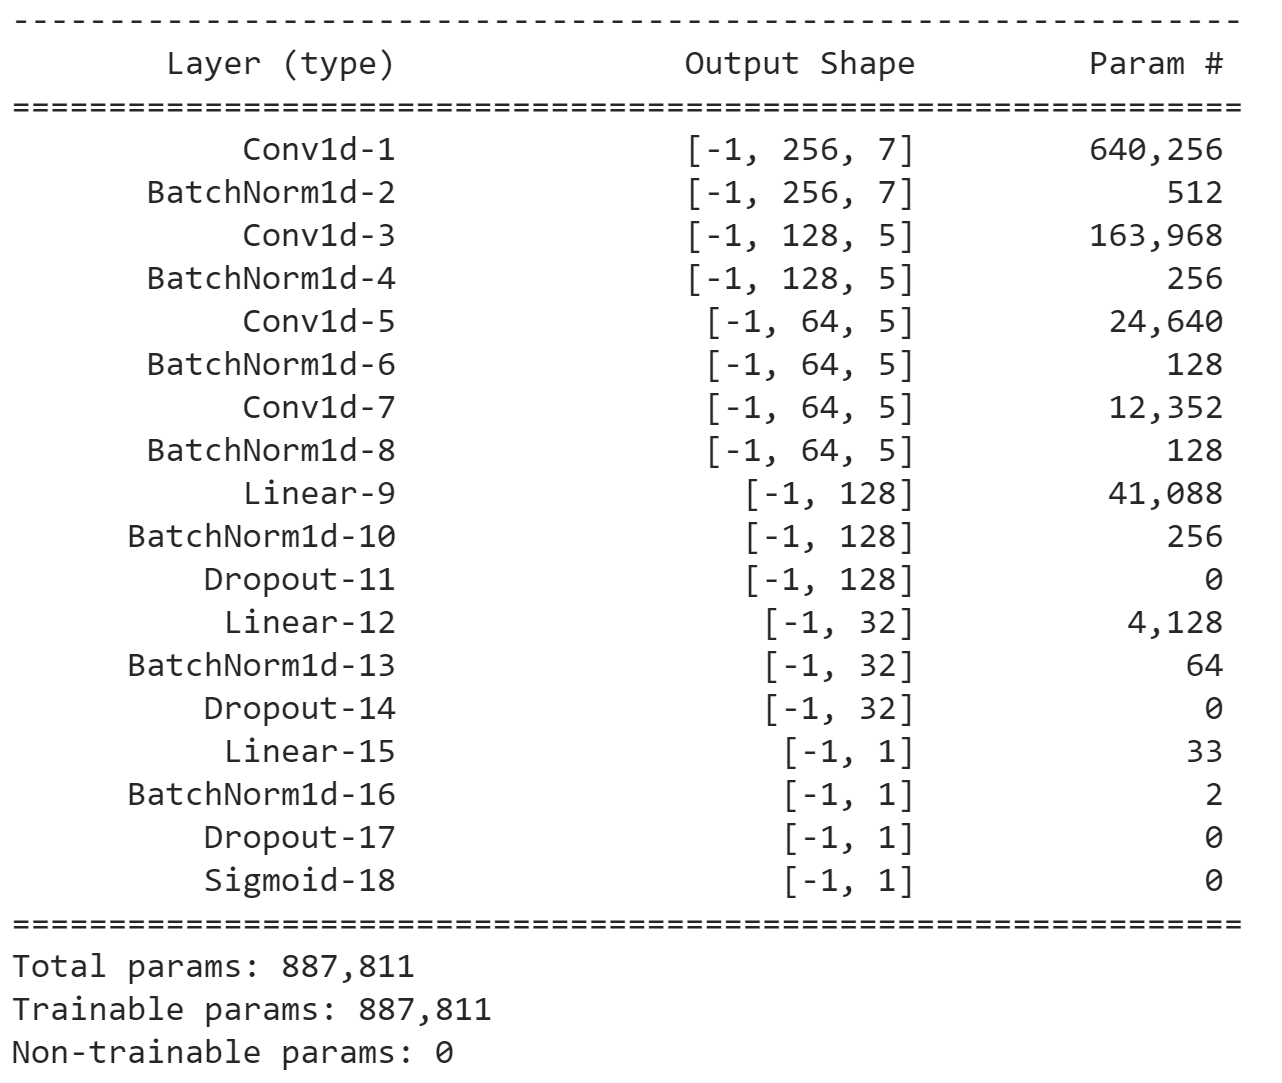
\includegraphics[width=1\linewidth]{report/img/network_summary.png}
  \caption{Model summary of CNN}
  \label{fig:cnn_model_summary}
\end{figure}

\section{Confusion Matrices}
\label{appendix:b}
Due to the underlying code that was used for this project, there is an error when calculating the Precision/Recall scores and comparing them to Table \ref{table:results_k_fold}. As a result, it is advised to look at the aforementioned table for reference as these scores were rounded manually.

\textbf{Note: }\textit{The following subsection s consist of confusion matrices for each row in Table \ref{table:results_k_fold}, where the first subfigure is the confusion matrix for Logistic Regression and the second subfigure is the result for the Mean prediction (both scores were calculated using the test set). Furthermore, due to the training set not exactly fitting the amount of batches (meaning $n \mod b \neq 0$, with n being the size of the dataset and b being the batch size), the amount of values in the cells in the confusion matrices can differ between batch sizes.
}
\subsection{TF-IDF, Binary, without user meta-data and batch size equal to 512}

\begin{figure}[H]
\centering
\begin{subfigure}
  \centering
  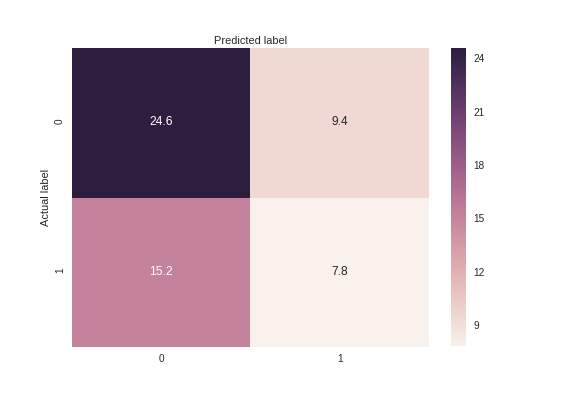
\includegraphics[width=1\linewidth]{report/img/conf_matrices/keywords_tfidf_binary_0_0_512_LR.png}
%   \caption{Confusion matrix LR}
  \label{fig:keywords_tfidf_binary_0_0_512_LR}
\end{subfigure}%
\begin{subfigure}
  \centering
  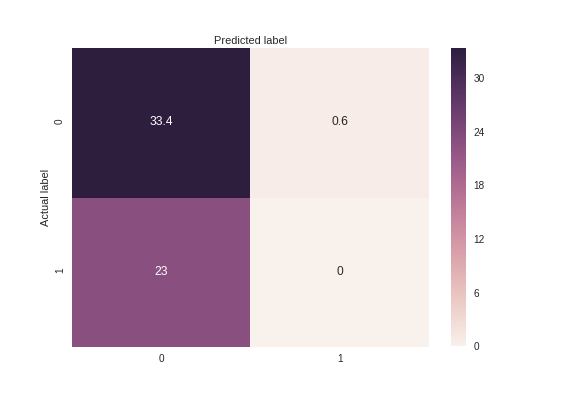
\includegraphics[width=1\linewidth]{report/img/conf_matrices/keywords_tfidf_binary_0_0_512_mean.png}
%   \caption{Confusion matrix mean}
  \label{fig:keywords_tfidf_binary_0_0_512_mean}
\end{subfigure}
\caption{Confusion matrices LR and Mean (see settings in Section title)}
\label{fig:keywords_tfidf_binary_0_0_512}
\end{figure}

\subsection{TF-IDF, Binary, with user meta-data and batch size equal to 512}

\begin{figure}[H]
\centering
\begin{subfigure}
  \centering
  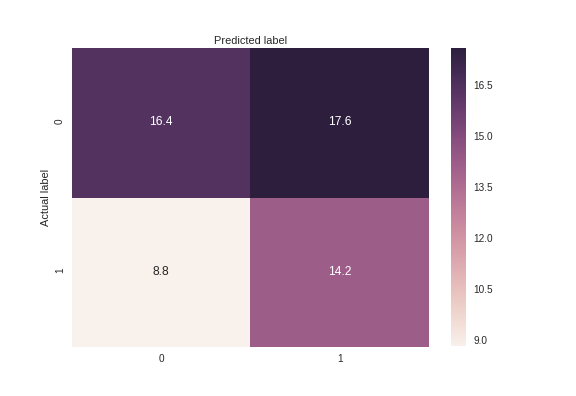
\includegraphics[width=1\linewidth]{report/img/conf_matrices/keywords_tfidf_binary_0_1_512_LR.png}
%   \caption{Confusion matrix LR}
  \label{fig:keywords_tfidf_binary_0_0_512_LR}
\end{subfigure}%
\begin{subfigure}
  \centering
  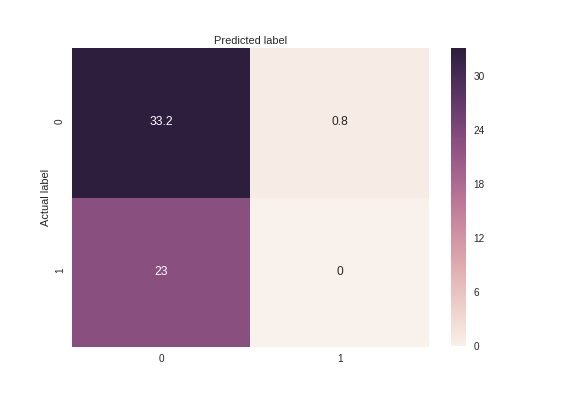
\includegraphics[width=1\linewidth]{report/img/conf_matrices/keywords_tfidf_binary_0_1_512_mean.png}
%   \caption{Confusion matrix mean}
  \label{fig:keywords_tfidf_binary_0_0_512_mean}
\end{subfigure}
\caption{Confusion matrices LR and Mean (see settings in Section title)}
\label{fig:keywords_tfidf_binary_0_0_512}
\end{figure}

\subsection{TF-IDF, Count, without user meta-data and batch size equal to 512}

\begin{figure}[H]
\centering
\begin{subfigure}
  \centering
  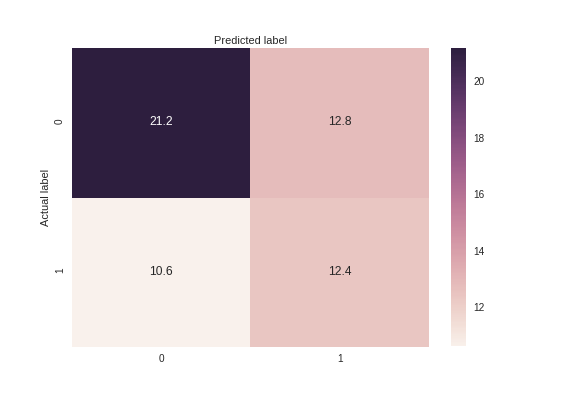
\includegraphics[width=1\linewidth]{report/img/conf_matrices/keywords_tfidf_count_0_0_512_LR.png}
%   \caption{Confusion matrix LR}
  \label{fig:keywords_tfidf_count_0_0_512_LR}
\end{subfigure}%
\begin{subfigure}
  \centering
  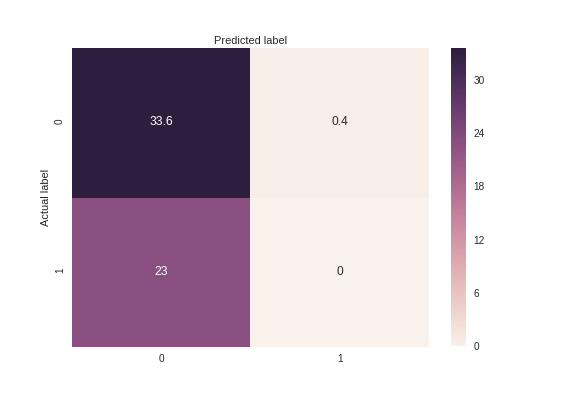
\includegraphics[width=1\linewidth]{report/img/conf_matrices/keywords_tfidf_count_0_0_512_mean.png}
%   \caption{Confusion matrix mean}
  \label{fig:keywords_tfidf_count_0_0_512_mean}
\end{subfigure}
\caption{Confusion matrices LR and Mean (see settings in Section title)}
\label{fig:keywords_tfidf_count_0_0_512}
\end{figure}

\subsection{TF-IDF, Count, with user meta-data and batch size equal to 512}

\begin{figure}[H]
\centering
\begin{subfigure}
  \centering
  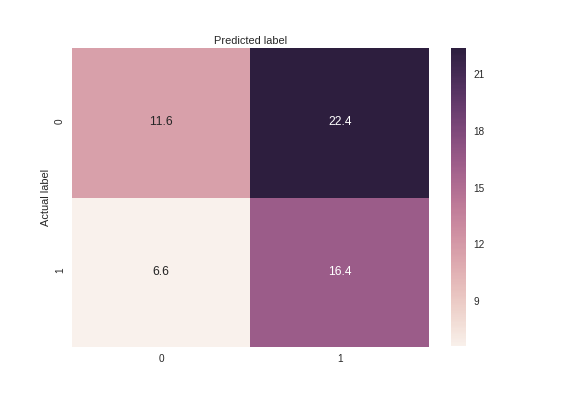
\includegraphics[width=1\linewidth]{report/img/conf_matrices/keywords_tfidf_count_0_1_512_LR.png}
%   \caption{Confusion matrix LR}
  \label{fig:keywords_tfidf_count_0_1_512_LR}
\end{subfigure}%
\begin{subfigure}
  \centering
  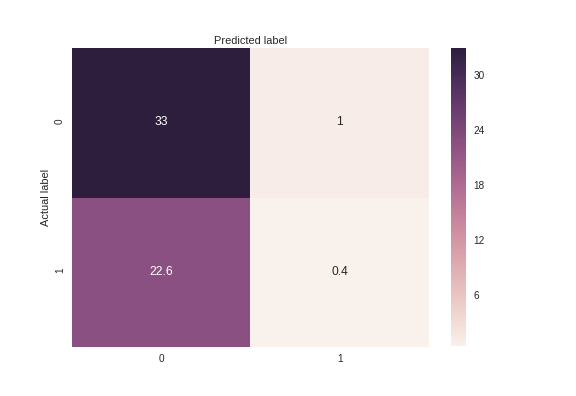
\includegraphics[width=1\linewidth]{report/img/conf_matrices/keywords_tfidf_count_0_1_512_mean.png}
%   \caption{Confusion matrix mean}
  \label{fig:keywords_tfidf_count_0_1_512_mean}
\end{subfigure}
\caption{Confusion matrices LR and Mean (see settings in Section title)}
\label{fig:keywords_tfidf_count_0_1_512}
\end{figure}

% --------------------------------

\subsection{Partial TF-IDF, Binary, without user meta-data and batch size equal to 512}

\begin{figure}[H]
\centering
\begin{subfigure}
  \centering
  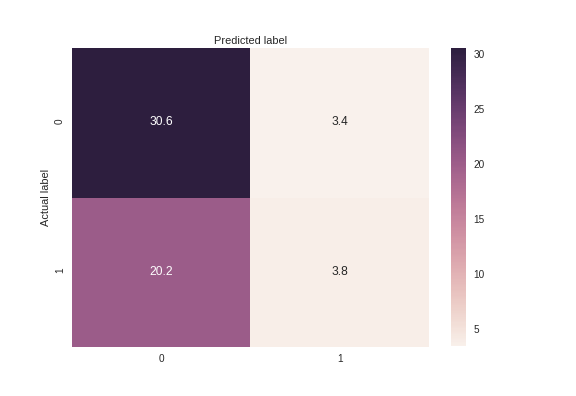
\includegraphics[width=1\linewidth]{report/img/conf_matrices/keywords_tfidf_p_binary_0_0_512_LR.png}
%   \caption{Confusion matrix LR}
  \label{fig:keywords_tfidf_p_binary_0_0_512_LR}
\end{subfigure}%
\begin{subfigure}
  \centering
  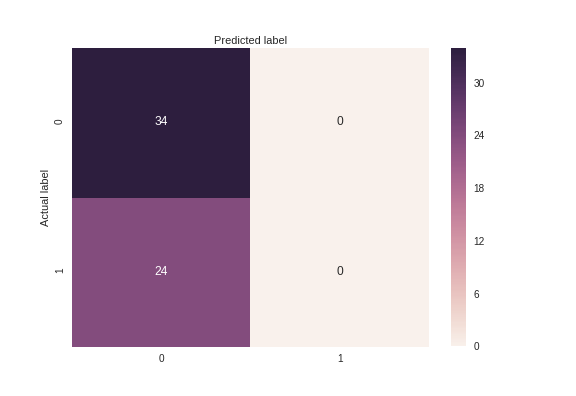
\includegraphics[width=1\linewidth]{report/img/conf_matrices/keywords_tfidf_p_binary_0_0_512_mean.png}
%   \caption{Confusion matrix mean}
  \label{fig:keywords_tfidf_p_binary_0_0_512_mean}
\end{subfigure}
\caption{Confusion matrices LR and Mean (see settings in Section title)}
\label{fig:keywords_tfidf_p_binary_0_0_512}
\end{figure}

\subsection{Partial TF-IDF, Binary, with user meta-data and batch size equal to 64}

\begin{figure}[H]
\centering
\begin{subfigure}
  \centering
  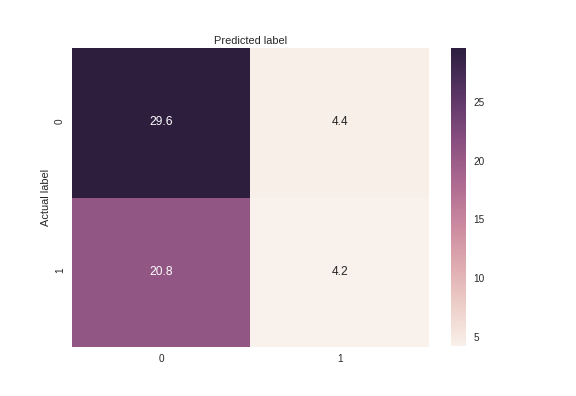
\includegraphics[width=1\linewidth]{report/img/conf_matrices/keywords_tfidf_p_binary_0_1_64_LR.png}
%   \caption{LR}
  \label{fig:keywords_tfidf_p_binary_0_1_64_LR}
\end{subfigure}%
\begin{subfigure}
  \centering
  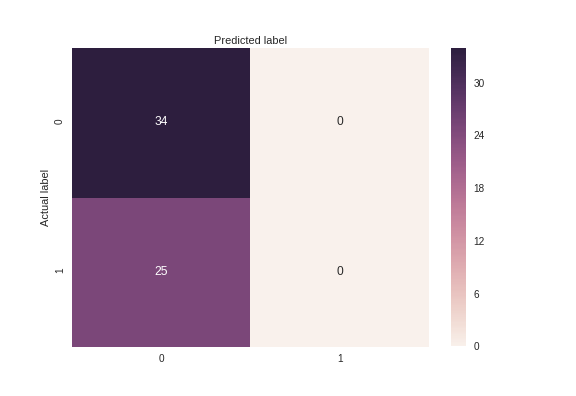
\includegraphics[width=1\linewidth]{report/img/conf_matrices/keywords_tfidf_p_binary_0_1_64_mean.png}
%   \caption{Mean}
  \label{fig:keywords_tfidf_p_binary_0_1_64_mean}
\end{subfigure}
\caption{Confusion matrices LR and Mean (see settings in Section title)}
\label{fig:keywords_tfidf_p_binary_0_1_64}
\end{figure}

\subsection{Partial TF-IDF, Count, without user meta-data and batch size equal to 256}
\label{app:b_best}

\begin{figure}[H]
\centering
\begin{subfigure}
  \centering
  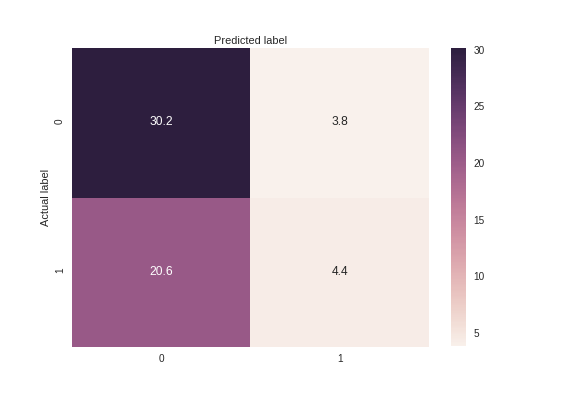
\includegraphics[width=1\linewidth]{report/img/conf_matrices/keywords_tfidf_p_count_0_0_256_LR.png}
%   \caption{Confusion matrix LR}
  \label{fig:keywords_tfidf_p_count_0_0_256_LR}
\end{subfigure}%
\begin{subfigure}
  \centering
  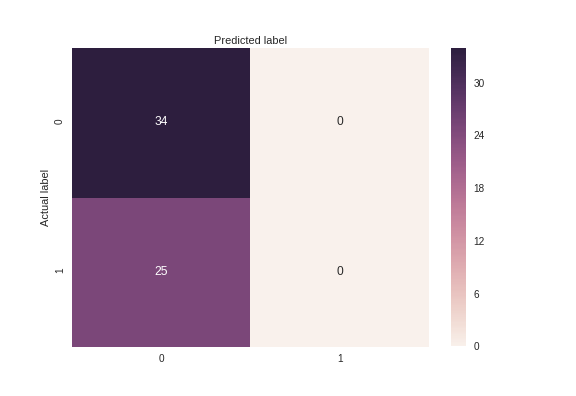
\includegraphics[width=1\linewidth]{report/img/conf_matrices/keywords_tfidf_p_count_0_0_256_mean.png}
%   \caption{Confusion matrix mean}
  \label{fig:keywords_tfidf_p_count_0_0_256_mean}
\end{subfigure}
\caption{Confusion matrices LR and Mean (see settings in Section title)}
\label{fig:keywords_tfidf_p_count_0_0_256}
\end{figure}

\subsection{Partial TF-IDF, Count, with user meta-data and batch size equal to 512}

\begin{figure}[H]
\centering
\begin{subfigure}
  \centering
  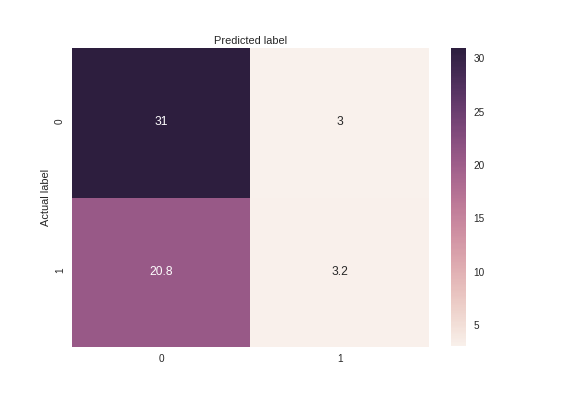
\includegraphics[width=1\linewidth]{report/img/conf_matrices/keywords_tfidf_p_count_0_1_512_LR.png}
%   \caption{Confusion matrix LR}
  \label{fig:keywords_tfidf_p_count_0_1_512_LR}
\end{subfigure}%
\begin{subfigure}
  \centering
  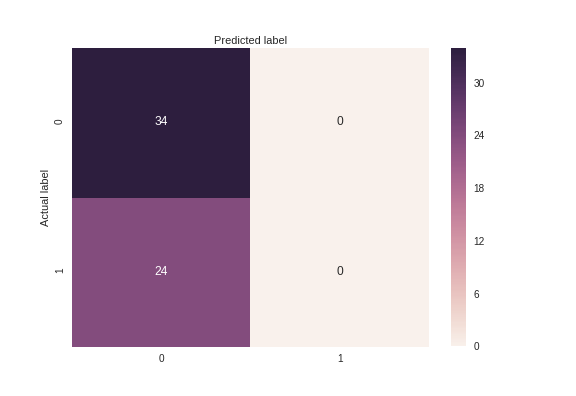
\includegraphics[width=1\linewidth]{report/img/conf_matrices/keywords_tfidf_p_count_0_1_512_mean.png}
%   \caption{Confusion matrix mean}
  \label{fig:keywords_tfidf_p_count_0_1_512_mean}
\end{subfigure}
\caption{Confusion matrices LR and Mean (see settings in Section title)}
\label{fig:keywords_tfidf_p_count_0_1_512}
\end{figure}

% Please add the following required packages to your document preamble:
% \usepackage{lscape}
% Please add the following required packages to your document preamble:
% \usepackage{lscape}
% \begin{landscape}

% \end{landscape}


\end{document}
